\documentclass[12pt]{article}
\usepackage{hyperref}
\usepackage{listings}
\usepackage[margin=1in]{geometry}
\usepackage{enumitem}
\usepackage{multicol}
\usepackage{array}
\usepackage{titlesec}
\usepackage{helvet}
\renewcommand{\familydefault}{\sfdefault}
\usepackage{amsmath}     % For math equations
\usepackage{amssymb}     % For advanced math symbols
\usepackage{amsfonts} % For math fonts
\usepackage{gvv}
\usepackage{esint}
\usepackage[utf8]{inputenc}
\usepackage{graphicx}
\usepackage{pgfplots}
\pgfplotsset{compat=1.18}
\titleformat{\section}{\bfseries\large}{\thesection.}{1em}{}
\setlength{\parindent}{0pt}
\setlength{\parskip}{6pt}
\usepackage{multirow}

\usepackage{fancyhdr}     % For custom headers and footers

\pagestyle{fancy}         % Use the fancy page style
\fancyhf{}                % Clear existing header/footer

% Header customization
\renewcommand{\headrulewidth}{0.4pt}          % Horizontal line at top
\fancyhead[L]{\textbf{GATE 2016}}                       % Page number on left
\fancyhead[R]{\textbf{ENGINEERING SCIENCES – XE}}  % Custom text on right
\cfoot{\thepage}

\usepackage[siunitx,RPvoltages]{circuitikz}
\usepackage{tikz}
\usepackage{float}
\usepackage{caption}

\begin{document}

\begin{enumerate}

\item[] \textbf{Q.1 - Q.5 carry one mark each}

  \item The chairman requested the aggrieved shareholders to \_\_\_\_\_\_\_\_\_ him.
  \begin{multicols}{4}
  \begin{enumerate}
    \item bare with
    \item bore with
    \item bear with
    \item bare
  \end{enumerate}
  \end{multicols}
  (GATE XE 2016)

  \item Identify the correct spelling out of the given options:
  \begin{multicols}{4}
  \begin{enumerate}
    \item Managable
    \item Manageable
    \item Manageble
    \item Managible
  \end{enumerate}
  \end{multicols}
  (GATE XE 2016)

  \item Pick the odd one out in the following: \\
  13, 23, 33, 43, 53
  \begin{multicols}{4}
  \begin{enumerate}
    \item 23
    \item 33
    \item 43
    \item 53
  \end{enumerate}
  \end{multicols}
  (GATE XE 2016)

  \item R2D2 is a robot. R2D2 can repair aeroplanes. No other robot can repair aeroplanes. \\
  Which of the following can be logically inferred from the above statements?
  \begin{enumerate}
    \item R2D2 is a robot which can only repair aeroplanes.
    \item R2D2 is the only robot which can repair aeroplanes.
    \item R2D2 is a robot which can repair only aeroplanes.
    \item Only R2D2 is a robot.
  \end{enumerate}
  (GATE XE 2016)

  \item If $|9y-6|=3$, then $y^2 - \frac{4y}{3}$ is \_\_\_\_\_\_
  \begin{multicols}{4}
  \begin{enumerate}
    \item 0
    \item $+\tfrac{1}{3}$
    \item $-\tfrac{1}{3}$
    \item undefined
  \end{enumerate}
  \end{multicols}
  (GATE XE 2016)

  \item The following graph represents the installed capacity for cement production (in tonnes) and the actual production (in tonnes) of nine cement plants of a cement company. Capacity utilization of a plant is defined as ratio of actual production of cement to installed capacity. A plant with installed capacity of at least 200 tonnes is called a large plant and a plant with lesser capacity is called a small plant. The difference between total production of large plants and small plants, in tonnes is

\begin{figure}[H]
    \centering
    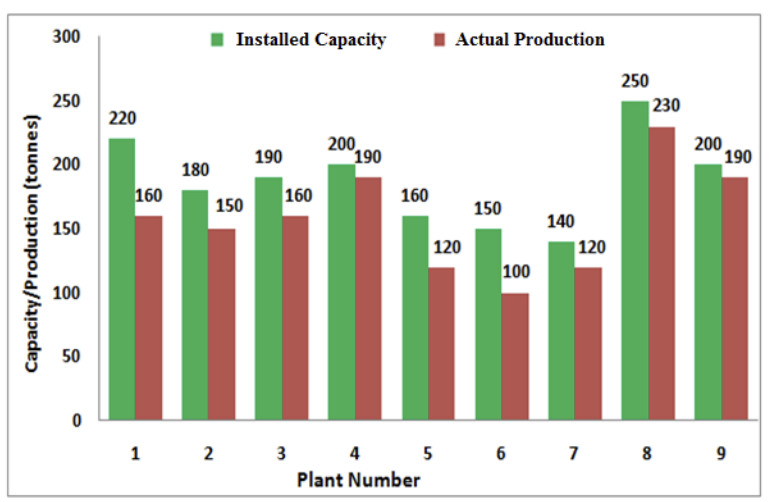
\includegraphics[width=0.7\columnwidth]{figs/ass3_0_q6.png}
    \caption{}
    \label{fig:placeholder}
\end{figure}
(GATE XE 2016)

\item A poll of students appearing for masters in engineering indicated that 60\% of the students believed that mechanical engineering is a profession unsuitable for women. A research study on women with masters or higher degrees in mechanical engineering found that 99\% of such women were successful in their professions. 

Which of the following can be logically inferred from the above paragraph?

\begin{enumerate}
    \item Many students have misconceptions regarding various engineering disciplines. 
    \item Men with advanced degrees in mechanical engineering believe women are well suited to be mechanical engineers. 
    \item Mechanical engineering is a profession well suited for women with masters or higher degrees in mechanical engineering. 
    \item The number of women pursuing higher degrees in mechanical engineering is small.
\end{enumerate}
(GATE XE 2016)

\item Sourya committee had proposed the establishment of Sourya Institutes of Technology (SITs) in line with Indian Institutes of Technology (IITs) to cater to the technological and industrial needs of a developing country.  

Which of the following can be logically inferred from the above sentence?  

Based on the proposal,  
(i) In the initial years, SIT students will get degrees from IIT.  
(ii) SITs will have a distinct national objective.  
(iii) SIT like institutions can only be established in consultation with IIT.  
(iv) SITs will serve technological needs of a developing country.  

\begin{multicols}{2}
\begin{enumerate}
    \item (iii) and (iv) only. 
    \item (i) and (iv) only. 
    \item (ii) and (iv) only. 
    \item (ii) and (iii) only. 
\end{enumerate}
\end{multicols}

(GATE XE 2016)  

\item Shaquille O'Neal is a 60\% career free throw shooter, meaning that he successfully makes 60 free throws out of 100 attempts on average. What is the probability that he will successfully make exactly 6 free throws in 10 attempts?  

\begin{multicols}{4}
\begin{enumerate}
    \item 0.2508
    \item 0.2816
    \item 0.2934
    \item 0.6000
\end{enumerate}
\end{multicols}

(GATE XE 2016)  

\item The numeral in the units position of $211^{870} + 146^{127} \times 3^{424}$ is \_\_\_\_. 

(GATE XE 2016)
\end{enumerate}

\newpage

\begin{center}
    {\Large \textbf{A : ENGINEERING MATHEMATICS (COMPULSORY)}}
\end{center}

\begin{enumerate}
\item[] \textbf{Q.1 - Q.7 carry one mark each.}

\item A company records heights of all employees. Let $X$ and $Y$ denote the errors in the average height of male and female employees respectively. Assume that $X \sim N(0,4)$ and $Y \sim N(0,9)$ and they are independent. Then the distribution of $Z = (X+Y)/2$ is  

\begin{multicols}{4}
\begin{enumerate}
    \item $N(0,6.5)$  
    \item $N(0,3.25)$  
    \item $N(0,2)$  
    \item $N(0,1)$  
\end{enumerate}
\end{multicols}

(GATE XE 2016)  

\item The volume of the solid obtained by revolving the curve $y^{2} = x,\ 0 \leq x \leq 1$ around $y$-axis is  

\begin{multicols}{4}
\begin{enumerate}
    \item $\pi$  
    \item $2$  
    \item $\tfrac{\pi}{2}$  
    \item $\tfrac{\pi}{5}$  
\end{enumerate}
\end{multicols}

(GATE XE 2016)  

\item Let $y(x)$ be the solution of the initial value problem  
$
\frac{dy}{dx} + 2xy = x, \quad y(0)=0.
$
Find the value of $\lim_{x \to \infty} y(x)$.  


(GATE XE 2016)  

\item Which of the following is a quasi-linear partial differential equation?  

\begin{enumerate}
    \item $\dfrac{\partial^{2}u}{\partial t^{2}} + u^{2} = 0$  
    \item $\left( \dfrac{\partial u}{\partial t} \right)^{2} + \dfrac{\partial u}{\partial x} = 0$  
    \item $\left( \dfrac{\partial u}{\partial t} \right)^{2} - \left( \dfrac{\partial u}{\partial x} \right)^{2} = 0$  
    \item $\left( \dfrac{\partial u}{\partial t} \right)^{4} - \left( \dfrac{\partial u}{\partial x} \right)^{3} = 0$  
\end{enumerate}

(GATE XE 2016)  

\item Let $P(x)$ and $Q(x)$ be the polynomials of degree $5$, generated by Lagrange and Newton interpolation methods respectively, both passing through given six distinct points on the $xy$-plane. Which of the following is correct?  

\begin{enumerate}
    \item $P(x) \equiv Q(x)$  
    \item $P(x) - Q(x)$ is a polynomial of degree $1$  
    \item $P(x) - Q(x)$ is a polynomial of degree $2$  
    \item $P(x) - Q(x)$ is a polynomial of degree $3$  
\end{enumerate}

(GATE XE 2016)  

\item The Laurent series of $f(z) = \frac{1}{z^3 - z^4}$ with center at $z=0$ in the region $|z| > 1$ is
\begin{multicols}{4}
\begin{enumerate}
\item $\sum_{n=0}^{\infty} z^{n-3}$
\item $-\sum_{n=0}^{\infty} \frac{1}{z^{n+4}}$
\item $\sum_{n=0}^{\infty} z^n$
\item $\sum_{n=0}^{\infty} \frac{1}{z^n}$
\end{enumerate}
\end{multicols}
(GATE XE 2016)

\item The value of the surface integral $\iint_{\Gamma} \vec{F} \cdot \vec{n} \, dS$ over the sphere $\Gamma$ given by $x^2+y^2+z^2=1$, where $\vec{F}=4x \, \hat{i} - z \, \hat{k}$ and $\vec{n}$ denotes the outward unit normal, is
\begin{multicols}{4}
\begin{enumerate}
\item $\pi$
\item $2\pi$
\item $3\pi$
\item $4\pi$
\end{enumerate}
\end{multicols}
(GATE XE 2016)


\item[] \textbf{Q.8 – Q.11 carry two marks each.}


\item A diagnostic test for a certain disease is $90\%$ accurate. That is, the probability of a person having (respectively, not having) the disease tested positive (respectively, negative) is $0.9$. Fifty percent of the population has the disease. What is the probability that a randomly chosen person has the disease given that the person tested negative?

(GATE XE 2016)

\item Let M = \myvec{0 & 1 \\ 0 & 1 }. Which of the following is correct?
\begin{enumerate}
\item Rank of $M$ is 1 and $M$ is not diagonalizable
\item Rank of $M$ is 2 and $M$ is diagonalizable
\item 1 is the only eigenvalue and $M$ is not diagonalizable
\item 1 is the only eigenvalue and $M$ is diagonalizable
\end{enumerate}
(GATE XE 2016)

\item Let $f(x) = 2x^3 - 3x^2 + 69,\;-5 \leq x \leq 5$. Find the point at which $f$ attains the global maximum.

(GATE XE 2016)

\item Calculate $\int_{C_1} \vec{F} \cdot d\vec{r} - \int_{C_2} \vec{F} \cdot d\vec{r}$, where $C_1 : \vec{r}(t) = (t, t^2)$ and $C_2 : \vec{r}(t) = (t, \sqrt{t}),$ \; t  varying from  0 to 1 and $\vec{F} = xy \, \hat{j}$.

(GATE XE 2016)
\end{enumerate}

\begin{center}
    \textbf{END OF SECTION - A}
\end{center}

\newpage

\begin{center}
    {\Large \textbf{B : FLUID MECHANICS}}
\end{center}

\begin{enumerate}
\item[] \textbf{Q.1 - Q.9 carry one mark each.}

\item In the parallel-plate configuration shown, steady-flow of an incompressible Newtonian fluid is established by moving the top plate with a constant speed, $U_0 = 1 \,\text{m/s}$. If the force required on the top plate to support this motion is $0.5 \,\text{N}$ per unit area (in $\text{m}^2$) of the plate then the viscosity of the fluid between the plates is \_\_\_\_\_\_\_ $N\cdot s/m^2$.

\begin{figure}[H]
    \centering
    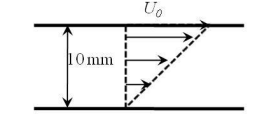
\includegraphics[width=0.5\columnwidth]{figs/ass3_b_q1.png}
    \caption{}
    \label{fig:placeholder}
\end{figure}
(GATE XE 2016)

\item For a newly designed vehicle by some students, volume of fuel consumed per unit distance travelled ($q_f$ in m$^3$/m) depends upon the viscosity ($\mu$) and density ($\rho$) of the fuel and, speed ($U$) and size ($L$) of the vehicle as
$$
q_f = C \frac{\rho U^2 L}{\mu^3}
$$
where $C$ is a constant. The dimensions of the constant $C$ are
\begin{multicols}{4}
\begin{enumerate}
\item $M^0 L^0 T^0$
\item $M^2 L^{-1} T^{-1}$
\item $M^2 L^{-5} T^{-1}$
\item $M^{-2} L T$
\end{enumerate}
\end{multicols}
(GATE XE 2016)

\item A semi-circular gate of radius $1\,\text{m}$ is placed at the bottom of a water reservoir as shown in figure below. The hydrostatic force per unit width of the cylindrical gate in $y$-direction is \_\_\_\_\_\_\_ kN. The gravitational acceleration, $g = 9.8\,\text{m/s}^2$ and density of water $= 1000\,\text{kg/m}^3$.

\begin{figure}[H]
    \centering
    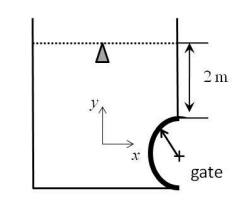
\includegraphics[width=0.7\columnwidth]{figs/ass3_b_q3.png}
    \caption{}
    \label{fig:placeholder}
\end{figure}
(GATE XE 2016)

\item Velocity vector in m/s for a 2-D flow is given in Cartesian coordinate $(x,y)$ as 
$
\vec{V} = \left(\tfrac{x^2}{4} \, \hat{i} - \tfrac{xy}{2} \, \hat{j}\right).
$
Symbols bear usual meaning. At a point in the flow field, the $x$- and $y$-components of the acceleration vector are given as $1\,\text{m/s}^2$ and $-0.5\,\text{m/s}^2$, respectively. The velocity magnitude at that point is \_\_\_\_ m/s.

(GATE XE 2016)

\item If $\phi(x,y)$ is velocity potential and $\psi(x,y)$ is stream function for a 2-D, steady, incompressible and irrotational flow, which one of the followings is incorrect?  
\begin{multicols}{2}
\begin{enumerate}
\item $\left(\frac{dy}{dx}\right)_{\phi = \text{const.}} =- \frac{1}{\left(\frac{dy}{dx}\right)_{\psi = \text{const.}}}$
\item $\frac{\partial^2 \psi}{\partial x^2} + \frac{\partial^2 \psi}{\partial y^2} = 0$
\item $\left(\frac{dy}{dx}\right)_{\phi = \text{const.}} =\frac{1}{ \left(\frac{dy}{dx}\right)_{\psi = \text{const.}}}$
\item $\frac{\partial^2 \phi}{\partial x^2} + \frac{\partial^2 \phi}{\partial y^2} = 0$
\end{enumerate}
\end{multicols}
(GATE XE 2016)

\item The flow field shown over a bluff body has considerably curved streamlines. A student measures pressures at points A, B, C, and D and denotes them as $P_A, P_B, P_C,$ and $P_D$ respectively. State which one of the following statements is true. The arrow indicates the freestream flow direction.  

\begin{figure}[H]
    \centering
    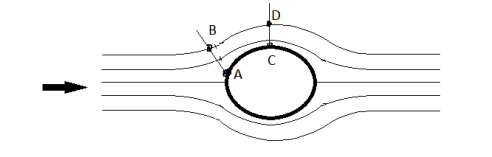
\includegraphics[width=0.5\columnwidth]{figs/ass3_b_q6.png}
    \caption{}
    \label{fig:placeholder}
\end{figure}
\begin{enumerate}
\item $P_A = P_B$ and $P_C > P_D$
\item $P_A > P_B$ and $P_C > P_D$
\item $P_A = P_B$ and $P_C < P_D$
\item $P_A > P_B$ and $P_C < P_D$
\end{enumerate}
(GATE XE 2016)

\item A 2-D incompressible flow is defined by its velocity components in m/s as $u = \frac{-cy}{x^2+y^2}$ and $v = \frac{cx}{x^2+y^2}$. If the value of the constant $c$ is equal to $0.1$ m$^2$/s, the numerical value of vorticity at the point $x=1$ m and $y=2$ m is \_\_\_\_\_\_ s$^{-1}$.  
(GATE XE 2016)

\item Two flow configurations are shown below for flow of incompressible, viscous flow. The inlet velocity for the diverging nozzle (Fig (i)) and free-stream velocity for flow past the bluff body (Fig (ii)) is constant. Points A and B are separation points and flow is laminar. The relation regarding velocity gradients at point A and B is (y is the direction normal to the surface at the point of separation).  

\begin{figure}[H]
    \centering
    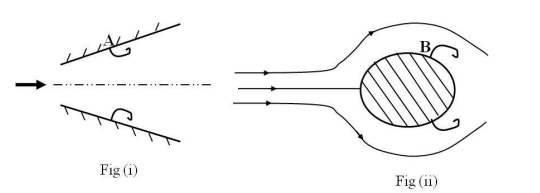
\includegraphics[width=0.7\columnwidth]{figs/ass3_b_q8.png}
    \caption{}
    \label{fig:placeholder}
\end{figure}
\begin{multicols}{4}
\begin{enumerate}
\item $(\frac{\partial u}{\partial y})_A$ = $(\frac{\partial u}{\partial y})_B$
\item $(\frac{\partial u}{\partial y})_A > (\frac{\partial u}{\partial y})_B$
\item $(\frac{\partial u}{\partial y})_A < (\frac{\partial u}{\partial y})_B$
\item $(\frac{\partial^2 u}{\partial y^2})_A =(\frac{\partial^2 u}{\partial y^2})_B$
\end{enumerate}
\end{multicols}
(GATE XE 2016)

\item Consider a fully developed, steady, incompressible, 2-D, viscous channel flow with uniform suction and blowing velocity $v_0$, as shown in the figure given below. The centerline velocity of the channel is $10 \, \text{m/s}$ along the $x$-direction. If the value of $v_0$ at both the walls is $1 \, \text{m/s}$, the value of the $y$-component of velocity inside the flow field is \_\_\_\_ m/s.  

\begin{figure}[H]
    \centering
    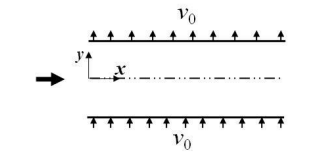
\includegraphics[width=0.5\columnwidth]{figs/ass3_b_q9.png}
    \caption{}
    \label{fig:placeholder}
\end{figure}

(GATE XE 2016)

\item[] \textbf{Q.10 - Q.22 carry two marks each.}

\item Exhaust from a kitchen goes into the atmosphere through a tapered chimney as shown. 
The area of cross-section of chimney at location-1 is twice of that at location-2. 
The flow can be assumed to be inviscid with constant exhaust density of $1 \, \text{kg/m}^3$ and acceleration due to gravity, $g = 9.8 \, \text{m/s}^2$. 
If the steady, uniform exhaust velocity at location-1 is $U = 1 \, \text{m/s}$, the pressure drop across the chimney is \_\_\_\_.  

\begin{figure}[H]
    \centering
    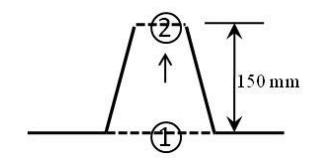
\includegraphics[width=0.5\columnwidth]{figs/ass3_b_q10.png}
    \caption{}
    \label{fig:placeholder}
\end{figure}

(GATE XE 2016)

\item A jet of diameter $20 \, \text{mm}$ and velocity $6 \, \text{m/s}$ coming out of a water-tank standing on a frictionless cart hits a vane and gets deflected at an angle $45^\circ$ as shown. 
The density of water is $1000 \, \text{kg/m}^3$. Neglect all minor and viscous losses. 
If the cart remains stationary, the magnitude of tension in the supporting string connected to the wall is \_\_\_\_ N.  

\begin{figure}[H]
    \centering
    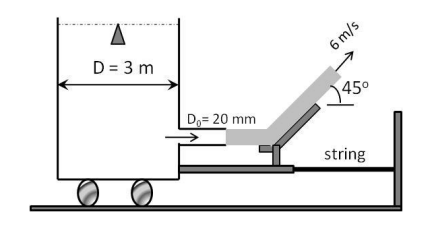
\includegraphics[width=0.5\columnwidth]{figs/ass3_b_q11.png}
    \caption{}
    \label{fig:placeholder}
\end{figure}

(GATE XE 2016)

\item A block is floating at the oil-water interface as shown. The density of oil is two-thirds of that of water. Given that the density of the block is $800 \, \text{kg/m}^3$ and that of water is $1000 \, \text{kg/m}^3$, the fraction of the total height of block in oil is \_\_\_\_.  

\begin{figure}[H]
    \centering
    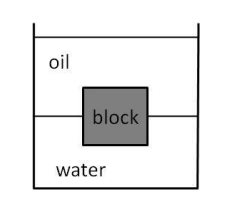
\includegraphics[width=0.5\columnwidth]{figs/ass3_b_q12.png}
    \caption{}
    \label{fig:placeholder}
\end{figure}

(GATE XE 2016)

\item A horizontal pipe is feeding water into a reservoir from the top with a time-dependent volumetric flow-rate, $Q \, (\text{m}^3/\text{h}) = 1 + 0.1 t$ where $t$ is time in hours. The area of the base of the reservoir is $0.5 \, \text{m}^2$. Assuming that initially the reservoir was empty, the height of the water level in the reservoir after 60 minutes is \_\_\_\_ m.  

(GATE XE 2016)

\item Velocity field of a 2-D steady flow is provided as $\vec{V} = c[(x^2 - y^2)\hat{i} - 2cxy\hat{j}]$.  
The equation of the streamlines of this flow is  

\begin{multicols}{2}
\begin{enumerate}
\item $x^2 y - \dfrac{y^3}{3} = \text{Constant}$  
\item $xy^2 - \dfrac{x^3}{3} = \text{Constant}$  
\item $xy - \dfrac{y^3}{3} = \text{Constant}$  
\item $x^2 y - \dfrac{y^2}{3} = \text{Constant}$  
\end{enumerate}
\end{multicols}

(GATE XE 2016)

\item Velocity potential and stream function in polar coordinates $(r, \theta)$ for a potential flow over a cylinder with radius $R$ is given as $\phi = U_{\infty} \left( r + \dfrac{R^2}{r} \right) \cos \theta$ and $\psi = U_{\infty} \left( r - \dfrac{R^2}{r} \right) \sin \theta$, respectively.  

Here, $U_{\infty}$ denotes uniform freestream velocity, and $\theta$ is measured counter clockwise. How does the velocity magnitude, $q$, over the surface of the cylinder vary?  

\begin{figure}[H]
    \centering
    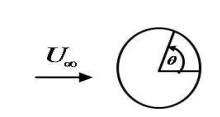
\includegraphics[width=0.5\columnwidth]{figs/ass3_b_q15.png}
    \caption{}
    \label{fig:placeholder}
\end{figure}

\begin{multicols}{2}
\begin{enumerate}
\item $q = 2U_{\infty} \cos \theta$  
\item $q = 2U_{\infty} \sin 2\theta$  
\item $q = U_{\infty} \cos 2\theta$  
\item $q = 2U_{\infty} \sin \theta$  
\end{enumerate}
\end{multicols}

(GATE XE 2016)

\item Consider a laminar flow over a flat plate of length $L = 1 \, \text{m}$. The boundary layer thickness at the end of the plate is $\delta_w$ for water, and $\delta_a$ for air for the same freestream velocity. If the kinematic viscosities of water and air are $1 \times 10^{-6} \, \text{m}^2/\text{s}$ and $1.6 \times 10^{-5} \, \text{m}^2/\text{s}$, respectively, the numerical value of the ratio $\dfrac{\delta_w}{\delta_a}$ is \_\_\_\_.  

(GATE XE 2016)

\item Prototype of a dam spillway (a structure used for controlled release of water from the dam) has characteristic length of $20 \, \text{m}$ and characteristic velocity of $2 \, \text{m/s}$. A small model is constructed by keeping Froude number same for dynamic similarity between prototype and the model. What is the minimum length-scale ratio between prototype and the model such that the minimum Reynolds' number for the model is 100? The density of water is $1000 \, \text{kg/m}^3$ and viscosity is $10^{-3} \, \text{Pa·s}$.  

\begin{multicols}{4}
\begin{enumerate}
\item $1.8 \times 10^{-4}$
\item $1 \times 10^{-4}$
\item $1.8 \times 10^{-3}$
\item $9.1 \times 10^{-4}$
\end{enumerate}
\end{multicols}

(GATE XE 2016)

\item An orifice meter, having orifice diameter of $d = \dfrac{20}{\sqrt{\pi}} \, \text{mm}$ is placed in a water pipeline having flow rate, $Q_{\text{act}} = 3 \times 10^{-4} \, \text{m}^3/\text{s}$. The ratio of orifice diameter to pipe diameter is $0.6$. The contraction coefficient is also $0.6$. The density of water is $1000 \, \text{kg/m}^3$. If the pressure drop across the orifice plate is $43.5 \, \text{kPa}$, the discharge coefficient of the orifice meter at this flow Reynolds number is \_\_\_\_.  

(GATE XE 2016)

\item Consider the following figures shown below. The objects are marked as A1, A2, B1, B2 and C1, C2 and the flow directions over these objects are shown by the respective arrow placed to the left of the object. Freestream velocities are same for all the cases. Amongst these objects, A1, A2, B1 and C1 are having smooth surfaces while B2 and C2 are having rough surfaces. Reynolds number is such that flow over rough surfaces becomes turbulent and flow over smooth surfaces can be considered laminar. All the airfoils can be considered as thin slender airfoils.  

Among the statements (i) to (vi) made about the drag of these objects, which is/are correct?  


(i) Drag of Object A1 is less than drag of Object A2.

(ii) Drag of Object A1 and A2 are same.  

(iii) Drag of Object B1 is more than drag of Object B2.

(iv) Drag of Object B2 is more than drag of Object B1.  

(v) Drag of Object C1 is more than drag of Object C2.  

(vi) Drag of Object C2 is more than drag of Object C1.  

\begin{figure}[H]
    \centering
    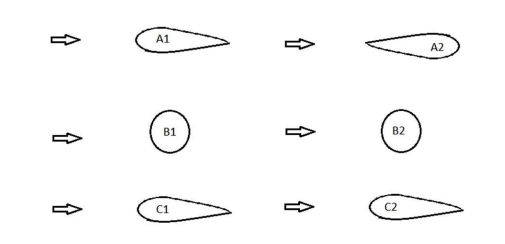
\includegraphics[width=0.5\columnwidth]{figs/ass3_b_q19.png}
    \caption{}
    \label{fig:placeholder}
\end{figure}


\begin{multicols}{4}
\begin{enumerate}
\item (i), (iii) \& (vi)
\item (ii), (iii) \& (vi)
\item (i), (iii) \& (v)
\item (i), (iv) \& (vi)
\end{enumerate}
\end{multicols}

(GATE XE 2016)

\item Consider 2-D, steady, incompressible, fully developed flow of viscous, Newtonian fluid through two stationary parallel plates, in Cartesian co-ordinate $(x,y,z)$ system. Assume plates are very long in $x$-direction, wide in $z$-direction (also there is no variation of velocity in $z$-direction) and distance between them is $2h$. The velocity in such a channel is given as  
$ U = U_{\text{max}} \left(1 - \frac{y^2}{h^2}\right) $
The origin $y=0$ is located at the center between the plates. If $h = 48 \, \text{mm}$ and $U_{\text{max}} = 100 \, \text{mm/s}$, difference between values of stream functions passing through $y=0$ and $y = h/2$ is \_\_\_\_ mm$^2$/s.  

(GATE XE 2016)

\item A pump is used to deliver water to an overhead tank at a flow rate of 
$Q = 4 \times 10^{-3} \, \text{m}^3/\text{s}$. 
The pump adds 1.6 kW to water. If the density of water is 
$1000 \, \text{kg}/\text{m}^3$ and acceleration due to gravity is 
$10 \, \text{m}/\text{s}^2$, the pump head added to the flow is \_\_\_\_\_\_ m.

(GATE XE 2016)

\item Water is discharged at atmospheric pressure from a large reservoir through a long pipe of diameter $d$ and length $L$. The height of the free surface of the reservoir from the discharge point is $h$ meters. The Darcy’s friction factor of the pipe is $0.002$. Neglect the velocity inside the reservoir as the reservoir is very large. Given, $L = 20 \, \text{m}, \quad d = 40 \, \text{mm}, \quad \text{density of water} = 1000 \,\text{kg}/\text{m}^3, \quad \text{and flow rate is } Q = 4 \pi \times 10^{-3} \, \text{m}^3/\text{s}$
Assume gravitational acceleration, $g = 10 \, \text{m}/\text{s}^2$.  
The value of $h$ is \_\_\_\_\_\_ m.

(GATE XE 2016)

\end{enumerate}

\begin{center}
    \textbf{END OF SECTION - B}
\end{center}

\newpage

\begin{center}
    {\Large \textbf{C : MATERIALS SCIENCE}}
\end{center}

\begin{enumerate}
\item[] \textbf{Q.1 - Q.9 carry one mark each.}

\item Energy Dispersive Spectroscopy (EDS) in a typical scanning electron microscope enables
elemental identification by collecting and examining which of the following:
\begin{enumerate}
  \item Secondary electrons from the sample
  \item Back scattered electrons from the sample
  \item Characteristic X-rays from the sample
  \item Diffraction pattern from the sample
\end{enumerate}
(GATE XE 2016)

\item Which of the following rotational symmetry is forbidden in a perfectly periodic 3-dimensional lattice?
\begin{multicols}{4}
\begin{enumerate}
  \item 1-fold
  \item 3-fold
  \item 5-fold
  \item 6-fold
\end{enumerate}
\end{multicols}
(GATE XE 2016)

\item Which of the following thermodynamic properties shows a discontinuity during a second-order phase transition?
\begin{multicols}{2}
\begin{enumerate}
  \item Volume
  \item Enthalpy
  \item Entropy
  \item Heat capacity
\end{enumerate}
\end{multicols}
(GATE XE 2016)

\item Cross slip is easily promoted in metals having
\begin{multicols}{2}
\begin{enumerate}
  \item a low stacking fault energy.
  \item a low grain boundary energy.
  \item a high stacking fault energy.
  \item a high grain boundary energy.
\end{enumerate}
\end{multicols}
(GATE XE 2016)

\item For a typical metal at room temperature and atmospheric pressure, the Fermi energy is defined as the energy level for which the probability of occupancy is:
\begin{multicols}{4}
\begin{enumerate}
  \item 0
  \item 0.25
  \item 0.5
  \item 1
\end{enumerate}
\end{multicols}
(GATE XE 2016)

\item Number of elements in a tensor of rank 4 is \_\_\_\_\_\_.

(GATE XE 2016)

\item Which one of the following effects is the working principle of a thermocouple?
\begin{multicols}{4}
\begin{enumerate}
  \item Thomson
  \item Seebeck
  \item Peltier
  \item Meissner
\end{enumerate}
\end{multicols}
(GATE XE 2016)

\item At equilibrium, the maximum number of phases that can coexist in a ternary system at constant pressure is \_\_\_\_\_\_.

(GATE XE 2016)

\item Defect-free single crystal alumina (sapphire) is
\begin{multicols}{2}
\begin{enumerate}
  \item opaque and white.
  \item transparent.
  \item translucent.
  \item opaque and black.
\end{enumerate}
\end{multicols}
(GATE XE 2016)

\item[] \textbf{Q.10 - Q.22 carry two marks each.}

\item Match the following processes and the products obtained:  

\begin{table}[H]
\centering
\caption{}
\label{}
\begin{tabular}{ll}
P: Mechanical attrition & 1: Thin films \\
Q: Physical vapour deposition & 2: Plastics \\
R: Injection moulding & 3: Nanoparticles \\
S: Sintering & 4: Rails \\
 & 5: Carbide tools \\
\end{tabular}
\end{table}

\begin{multicols}{2}
\begin{enumerate}
  \item P-1, Q-2, R-3, S-5
  \item P-3, Q-1, R-2, S-5
  \item P-4, Q-1, R-3, S-2
  \item P-3, Q-4, R-1, S-2
\end{enumerate}
\end{multicols}
(GATE XE 2016)

\item In a diffraction experiment, monochromatic X-rays of wavelength $1.54 \, \text{\AA}$ are used to examine a material with a BCC structure. If the lattice parameter is $4.1 \, \text{\AA}$, the angular position $\theta$ of the first diffraction peak is \_\_\_\_\_\_\_ degrees.  

(GATE XE 2016)

\item The yield strength of a ferritic steel increases from 120 MPa to 150 MPa when the grain size is decreased from 256 $\mu$m to 64 $\mu$m. When the grain size is further reduced to 16 $\mu$m, the expected yield strength is \_\_\_\_\_\_ MPa.  

(GATE XE 2016)

\item A direct bandgap semiconductor has a bandgap of $1.8 \, \text{eV}$. The threshold value of the wavelength BELOW which this material will absorb radiation is \_\_\_\_\_\_\_ \AA.  

(Given: Planck’s constant, $h = 6.626 \times 10^{-34} \, \text{J s}$, the charge of an electron, $e = 1.6 \times 10^{-19} \, \text{C}$, and speed of light, $c = 3 \times 10^{8} \, \text{m s}^{-1}$)  

(GATE XE 2016)

\item A half cell consisting of pure Ni immersed in an aqueous solution containing Ni$^{2+}$ ions of unknown concentration, is galvanically coupled with another half cell consisting of pure Cd immersed in a 1 M aqueous solution of Cd$^{2+}$ ions. The temperature is 25 $^\circ$C and pressure is 1 atm. The electrode reduction potentials of Ni and Cd are $-0.250 \, \text{V}$ and $-0.403 \, \text{V}$, respectively. The voltage of the cell is found to be zero. The concentration of Ni$^{2+}$ in the solution is \_\_\_\_\_ $\times 10^{-6}$ M.  

(Given: Universal gas constant, $R = 8.31 \, \text{J mol}^{-1} \text{K}^{-1}$, Faraday’s constant, $F = 96500 \, \text{C mol}^{-1}$)  

(GATE XE 2016)

\item Match the type of magnetism given in Group 1 with the material given in Group 2:  

\begin{table}[H]
\centering
\caption{}
\label{}
\begin{tabular}{ll}
Group 1 & Group 2 \\
P: Ferromagnetic & 1: Nickel oxide \\
Q: Ferrimagnetic & 2: Sodium \\
R: Antiferromagnetic & 3: Magnetite \\
S: Paramagnetic & 4: Cobalt \\
\end{tabular}
\end{table}

\begin{multicols}{2}
\begin{enumerate}
  \item P-4, Q-3, R-1, S-2
  \item P-4, Q-1, R-3, S-2
  \item P-1, Q-2, R-4, S-3
  \item P-3, Q-2, R-1, S-4
\end{enumerate}
\end{multicols}
(GATE XE 2016)

\item Gallium is to be diffused into pure silicon wafer such that its concentration at a depth of $10^{-3} \, \text{cm}$ will be one half the surface concentration. Given that the diffusion coefficient ($D$) of gallium in silicon at $1355 \, ^\circ$C is $6 \times 10^{-11} \, \text{cm}^2 \, \text{s}^{-1}$, the time the silicon wafer should be heated in contact with gallium vapour at $1355 \, ^\circ$C is \underline{\hspace{2cm}} s.  

(Given: $erf(0.5) \approxeq 0.5$)  

(GATE XE 2016)

\item A batch of spherical titania nanoparticles, uniform in size, has a specific surface area of 125 m$^2$ g$^{-1}$. If the density of titania is 4.23 g cm$^{-3}$, the diameter of the particles is \_\_\_\_\_\_\_ nm.  

(GATE XE 2016)

\item Given the probability distribution function  
$$
f(x) = 
\begin{cases}
0.25x & \text{for } 1 \leq x \leq 3 \\
0 & \text{otherwise}
\end{cases}
$$
The probability that the random variable $x$ takes a value between 1 and $\sqrt{5}$ is \_\_\_\_\_\_\_.  

(GATE XE 2016)

\item In the vulcanization of 50 g of natural rubber, 10 g of sulfur is added. Assuming the mer to S ratio is 1:1, the maximum percentage of cross-linked sites that could be connected is \_\_\_\_\_\_\_ \%.  
(Given: atomic weight of S is 32 amu and molecular weight of a mer of natural rubber is 68 amu)  

(GATE XE 2016)

\item Match the heat treatment process of steels given in Group 1 with the microstructural feature given in Group 2:  

\begin{table}[H]
\centering
\caption{}
\label{}
\begin{tabular}{l l}
\textbf{Group 1} & \textbf{Group 2} \\
P: Quenching     & 1: Bainite \\
Q: Normalizing   & 2: Martensite \\
R: Tempering     & 3: Pearlite \\
S: Austempering  & 4: Iron carbide precipitates \\
                 & 5: Intermetallic precipitates \\
\end{tabular}
\end{table}

\begin{multicols}{2}
\begin{enumerate}
\item  P-2, Q-3, R-4, S-1 
\item  P-3, Q-4, R-5, S-1 
\item P-4, Q-1, R-5, S-3 
\item P-2, Q-5, R-4, S-3  
\end{enumerate}
\end{multicols}

(GATE XE 2016)

\item In the photoelectric effect, electrons are ejected  

\begin{enumerate}
\item at all wavelengths, as long as the intensity of the incident radiation is above a threshold value.  
\item at all wavelengths, as long as the intensity of the incident radiation is below a threshold value.  
\item at all intensities, as long as the wavelength of the incident radiation is below a threshold value.  
\item at all intensities, as long as the wavelength of the incident radiation is above a threshold value.  
\end{enumerate}

(GATE XE 2016)

\item The angle between [110] and [111] directions in the cubic system is \_\_\_\_\_\_
degrees.

(GATE XE 2016)


\end{enumerate}

\begin{center}
    \textbf{END OF SECTION - C}
\end{center}

\newpage

\begin{center}
    {\Large \textbf{D : SOLID MECHANICS}}
\end{center}

\begin{enumerate}
\item[] \textbf{Q.1 - Q.9 carry one mark each.}

\item A single degree of freedom vibrating system has mass of 5 kg, stiffness of 500 N/m and damping coefficient of 100 N-s/m. To make the system critically damped  
\begin{enumerate}
\item only the mass is to be increased by 1.2 times.  
\item only the stiffness is to be reduced to half.  
\item only the damping coefficient is to be doubled.  
\item no change in any of the system parameters is required.  
\end{enumerate}
(GATE XE 2016)

\item A ``L'' shaped robotic arm AB is connected to a motor at end A and a magnetic gripper at B as shown in the figure. If the arm is rotating with an angular velocity of 2 rad/s and an angular acceleration of 3 rad/s$^2$, the magnitude of the acceleration (in m/s$^2$) of the end B is  

\begin{figure}[H]
    \centering
    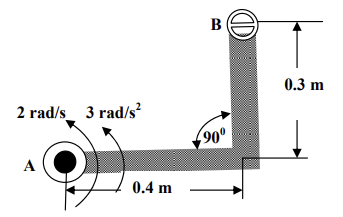
\includegraphics[width=0.5\columnwidth]{figs/ass3_d_q2.png}
    \caption{}
    \label{fig:placeholder}
\end{figure}
\begin{multicols}{4}
\begin{enumerate}
\item 2.0  
\item 2.5  
\item 5.0  
\item 6.0  
\end{enumerate}
\end{multicols}
(GATE XE 2016)

\item A block of weight 100 N is in static equilibrium on an inclined plane which makes an angle $15^\circ$ with the horizontal. The coefficient of friction between the inclined plane and the block is 0.3. The magnitude of friction force (in N) acting on the block is \_\_\_\_\_\_ .  

\begin{figure}[H]
    \centering
    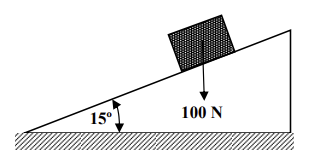
\includegraphics[width=0.5\columnwidth]{figs/ass3_d_q3.png}
    \caption{}
    \label{fig:placeholder}
\end{figure}
(GATE XE 2016)

\item The lower end $A$ of the rigid bar $AB$ is moving horizontally on the floor towards right with a constant velocity of $5 \ \text{m/s}$ and the point $B$ is sliding down the wall. The magnitude of the velocity of point $B$ at the instant $\theta = 30^\circ$ is 

\begin{figure}[H]
    \centering
    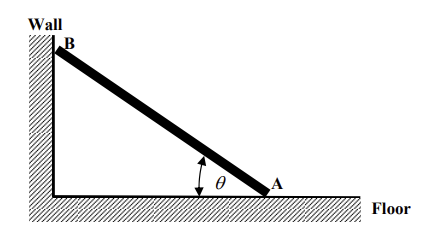
\includegraphics[width=0.5\columnwidth]{figs/ass3_d_q4.png}
    \caption{}
    \label{fig:placeholder}
\end{figure}

\begin{multicols}{4}
\begin{enumerate}
\item zero
\item 4.34 m/s
\item 7.25 m/s
\item 8.66 m/s
\end{enumerate}
\end{multicols}

(GATE XE 2016)

\item The state of plane stress at a point in a body is shown in the figure. The allowable shear stress of the material of the body is 200 MPa. According to the maximum shear stress theory of failure the maximum permissible value of $\sigma$ (in MPa) is \_\_\_\_\_\_

\begin{figure}[H]
    \centering
    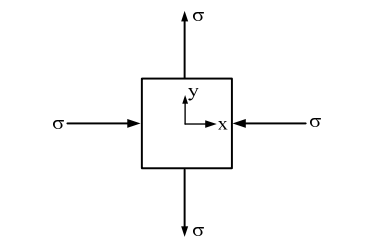
\includegraphics[width=0.5\columnwidth]{figs/ass3_d_q5.png}
    \caption{}
    \label{fig:placeholder}
\end{figure}

(GATE XE 2016)

\item For a slender steel column of circular cross-section the critical buckling load is $P_{cr}$. If the diameter of the column is doubled (keeping other material and geometrical parameters same), then the critical buckling load of the column is

\begin{multicols}{4}
\begin{enumerate}
\item $P_{cr}/16$
\item $8P_{cr}$
\item $2P_{cr}$
\item $16P_{cr}$
\end{enumerate}
\end{multicols}

(GATE XE 2016)

\item A closed thin cylindrical pressure vessel having an internal diameter of $1000 \ \text{mm}$ and a thickness of $10 \ \text{mm}$ is subjected to an internal pressure of $4 \ \text{MPa}$. The maximum shear stress (in MPa) induced in the cylinder is \_\_\_\_\_\_\_\_\_ (neglect the radial stress).

(GATE XE 2016)

\item A solid circular shaft subjected to pure torsion develops a maximum torsional shear stress of $120 \ \text{MPa}$. Keeping the torsional moment same, if the diameter of the shaft is doubled then the maximum shear stress (in MPa) induced in the shaft is \_\_\_\_\_\_\_\_\_.

(GATE XE 2016)

\item On a single straight track, a vehicle of mass $500 \ \text{kg}$ moving with a velocity of $25 \ \text{m/s}$ strikes another vehicle of mass $250 \ \text{kg}$ moving with a velocity $10 \ \text{m/s}$ in the same direction. After the impact, if both the vehicles stick together, the common velocity (in m/s) with which both the vehicles will move together is \_\_\_\_\_\_\_\_\_ 

(GATE XE 2016)


\item[] \textbf{Q.10 -- Q.22 carry two marks each.}

\item A system with three forces and a concentrated moment at $A$ is shown in the figure. The system is replaced by an equivalent force system with a single force and a single couple at point $O$. The magnitude (in N-m) of the equivalent couple at $O$ is \_\_\_\_\_\_\_\_\_

\begin{figure}[H]
    \centering
    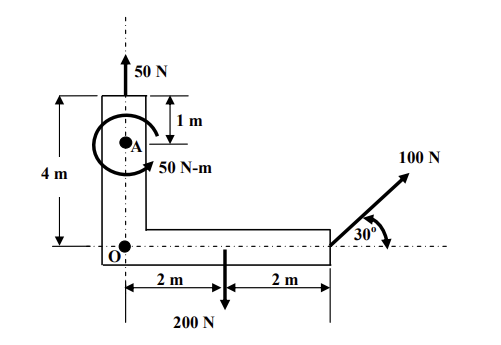
\includegraphics[width=0.5\columnwidth]{figs/ass3_d_q10.png}
    \caption{}
    \label{fig:placeholder}
\end{figure}

(GATE XE 2016)

\item A block $A$ on a smooth inclined plane is connected to block $B$ as shown in the figure using an inextensible cord which passes over a mass-less and friction-less pulley. Initially, the block $B$ is constrained to be at rest. If the constraint on block $B$ is released, the magnitude of velocity (in m/s) of the block $B$ after $2$ seconds from its release is \_\_\_\_\_\_\_\_\_ (assume $g=10 \ \text{m/s}^2$).

\begin{figure}[H]
    \centering
    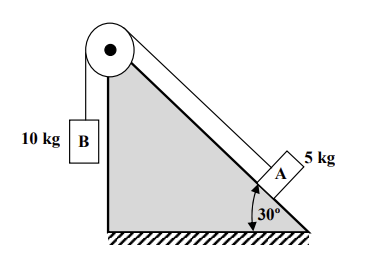
\includegraphics[width=0.5\columnwidth]{figs/ass3_d_q11.png}
    \caption{}
    \label{fig:placeholder}
\end{figure}

(GATE XE 2016)

\item The vibrating system shown in the figure carries a mass of $10 \ \text{kg}$ at the free end, where the static deflection is $1 \ \text{mm}$. This system is to be replaced by an equivalent vibrating spring mass system having equivalent mass of $2 \ \text{kg}$ (assume $g=10 \ \text{m/s}^2$). The natural frequency (in rad/s) and the stiffness (in kN/m) of the equivalent system respectively are

\begin{figure}[H]
    \centering
    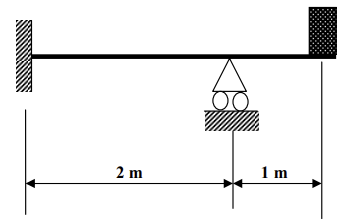
\includegraphics[width=0.5\columnwidth]{figs/ass3_d_q12.png}
    \caption{}
    \label{fig:placeholder}
\end{figure}

\begin{multicols}{4}
\begin{enumerate}
\item 10 and 20
\item 20 and 100
\item 100 and 20
\item 1000 and 20
\end{enumerate}
\end{multicols}

(GATE XE 2016)

\item A beam having flexural rigidity $EI$ and length $L$ is subjected to a concentrated end moment $M_0$ as shown in the figure. For $EI = 4 \times 10^3 \ \text{N-m}^2$, $L = 1 \ \text{m}$ and $M_0 = 8 \ \text{kN-m}$, the strain energy stored (in kN-m) in the beam and the rotation (in rad) at the free end respectively are

\begin{figure}[H]
    \centering
    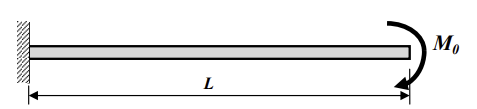
\includegraphics[width=0.5\columnwidth]{figs/ass3_d_q13.png}
    \caption{}
    \label{fig:placeholder}
\end{figure}

\begin{multicols}{4}
\begin{enumerate}
\item 8.00 and 0.02
\item 8.00 and 2.00
\item 8.00 and 0.04
\item 0.80 and 2.00
\end{enumerate}
\end{multicols}

(GATE XE 2016)

\item At a point $O$ on a metal sheet a square $OABC$ of a unit side length is drawn. The square undergoes a small uniform elastic deformation and deforms to $OA^*B^*C^*$ (dashed lines) as shown in the figure. All dimensions are in mm and the figure is not to scale. The normal strains $\varepsilon_x, \varepsilon_y$ and shear strain $\gamma_{xy}$ developed in the square respectively are

\begin{figure}[H]
    \centering
    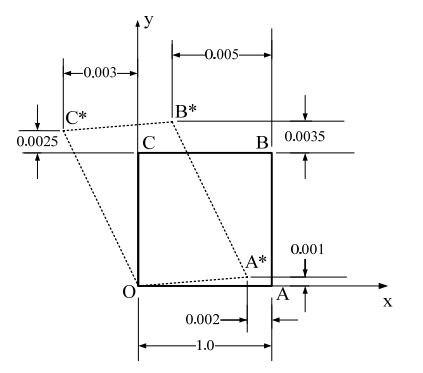
\includegraphics[width=0.5\columnwidth]{figs/ass3_d_q14.png}
    \caption{}
    \label{fig:placeholder}
\end{figure}

\begin{multicols}{2}
\begin{enumerate}
\item $-0.0020, \ 0.0025 \ \text{and} \ 0.0020$
\item $0.0020, \ -0.0025 \ \text{and} \ -0.0020$
\item $0.0025, \ -0.0020 \ \text{and} \ 0.0020$
\item $-0.0020, \ 0.0025 \ \text{and} \ -0.0020$
\end{enumerate}
\end{multicols}

(GATE XE 2016)

\item Mohr’s circle for the state of plane stress at a point is shown in the figure. Unit of stress is MPa and the circle is drawn not to scale. Which one of the following options (stress values in MPa) is true?

\begin{figure}[H]
    \centering
    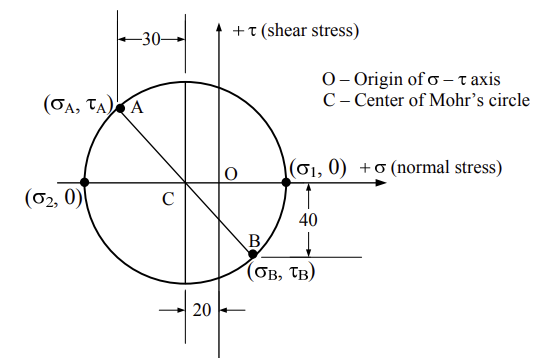
\includegraphics[width=0.5\columnwidth]{figs/ass3_d_q15.png}
    \caption{}
    \label{fig:placeholder}
\end{figure}

\begin{multicols}{2}
\begin{enumerate}
\item $\sigma_x = -50, \ \sigma_y = 10, \ \sigma_1 = 30, \ \sigma_2 = -70$
\item $\sigma_x = -50, \ \sigma_y = 20, \ \sigma_1 = 30, \ \sigma_2 = -50$
\item $\sigma_x = -30, \ \sigma_y = 30, \ \sigma_1 = 30, \ \sigma_2 = -10$
\item $\sigma_x = -20, \ \sigma_y = 10, \ \sigma_1 = 50, \ \sigma_2 = -30$
\end{enumerate}
\end{multicols}

(GATE XE 2016)

\item As shown in the figure, links $AB$ and $CD$ support the rigid member $BD$. Links $AB$ and $CD$ are made of aluminum alloy ($E = 100 \ \text{GPa}$) and each has a cross-sectional area of $100 \ \text{mm}^2$. All the members are pin connected and all the dimensions are in mm. Neglecting the weights of the members, the elongation (in mm) of the link $AB$ is \_\_\_\_\_\_\_\_\_

\begin{figure}[H]
    \centering
    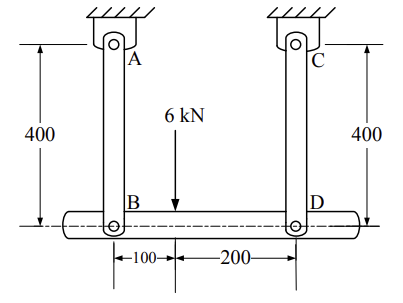
\includegraphics[width=0.5\columnwidth]{figs/ass3_d_q16.png}
    \caption{}
    \label{fig:placeholder}
\end{figure}

(GATE XE 2016)

\item Figure shows an elastic beam of constant flexural rigidity $EI$ and length $L$. The transverse deflection $v(x)$ for the beam is represented by the equation  
$v(x) = \frac{M_0 \left( x^3 - x^2 L \right)}{4EI \, L},$
where $M_0$ is the applied couple. If $L = 100 \ \text{mm}$ and $M_0 = 100 \ \text{N-mm}$, then the magnitude of the shear force (in N) at the middle of the beam (at $x = L/2$) is \_\_\_\_\_\_\_\_\_

\begin{figure}[H]
    \centering
    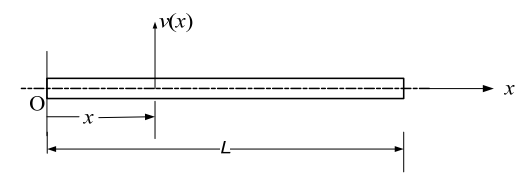
\includegraphics[width=0.8\columnwidth]{figs/ass3_d_q17.png}
    \caption{}
    \label{fig:placeholder}
\end{figure}

(GATE XE 2016)

\item Which one of the following represents the correct bending moment diagram of the beam $PQR$ loaded as shown in the figure?
\begin{figure}[H]
    \centering
    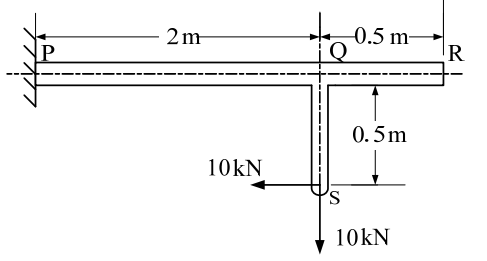
\includegraphics[width=0.5\columnwidth]{figs/ass3_d_q18.png}
    \caption{}
    \label{fig:placeholder}
\end{figure}

\begin{multicols}{2}
\begin{enumerate}

\item \begin{figure}[H]
    \centering
    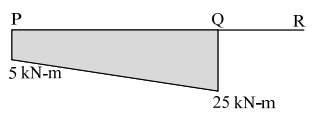
\includegraphics[width=0.8\columnwidth]{figs/ass3_d_q18_a.png}
    \caption{}
    \label{fig:placeholder}
\end{figure}

\item \begin{figure}[H]
    \centering
    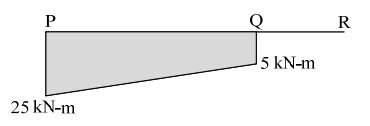
\includegraphics[width=0.8\columnwidth]{figs/ass3_d_q18_b.png}
    \caption{}
    \label{fig:placeholder}
\end{figure}

\item \begin{figure}[H]
    \centering
    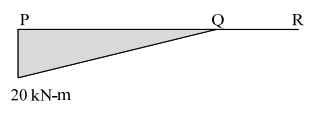
\includegraphics[width=0.8\columnwidth]{figs/ass3_d_q18_c.png}
    \caption{}
    \label{fig:placeholder}
\end{figure}

\item \begin{figure}[H]
    \centering
    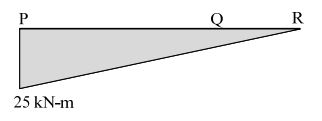
\includegraphics[width=0.8\columnwidth]{figs/ass3_d_q18_d.png}
    \caption{}
    \label{fig:placeholder}
\end{figure}
\end{enumerate}
    
\end{multicols}

(GATE XE 2016)

\item A point in a body is subjected to plane state of stress in $XY$ plane. If $\sigma_x = 140 \ \text{MPa}$, $\sigma_y = 60 \ \text{MPa}$ and the major principal stress is $150 \ \text{MPa}$, the magnitude of the in-plane shear stress $\tau_{xy}$ (in MPa) is

\begin{multicols}{4}
\begin{enumerate}
\item 75
\item 30
\item 40
\item 70
\end{enumerate}
\end{multicols}

(GATE XE 2016)

\item A $40 \ \text{mm}$ diameter rotor shaft of a helicopter transmits a torque $T = 0.16 \pi \ \text{kN-m}$ and a tensile force $P = 24 \pi \ \text{kN}$. The maximum tensile stress (in MPa) induced in the shaft is \_\_\_\_\_\_\_\_\_. Use the value of $\pi = 3.1416$.

\begin{figure}[H]
    \centering
    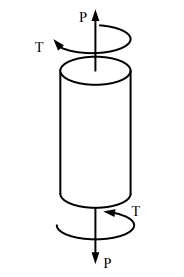
\includegraphics[width=0.3\columnwidth]{figs/ass3_d_q20.png}
    \caption{}
    \label{fig:placeholder}
\end{figure}

(GATE XE 2016)

\item A wooden block of length $400 \ \text{mm}$, width $50 \ \text{mm}$ and depth $100 \ \text{mm}$ is subjected to uniaxial load as shown in the figure. An inclined plane $ABCD$ is shown which makes an angle $\theta$ with the $XZ$ plane and the line $CD$ is parallel to the $Z$-axis. The normal stress on the plane $ABCD$ is $\sigma_{n1}$ when $\theta = 30^\circ$ and the normal stress on the plane $ABCD$ is $\sigma_{n2}$ when $\theta = 120^\circ$. The value of $\dfrac{\sigma_{n2}}{\sigma_{n1}}$ is \_\_\_\_\_\_\_\_\_.

\begin{figure}[H]
    \centering
    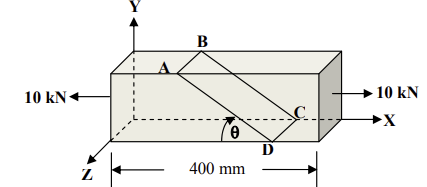
\includegraphics[width=0.5\columnwidth]{figs/ass3_d_q21.png}
    \caption{}
    \label{fig:placeholder}
\end{figure}

(GATE XE 2016)

\item For the truss shown in the figure, which one of the following statements is true?

\begin{figure}[H]
    \centering
    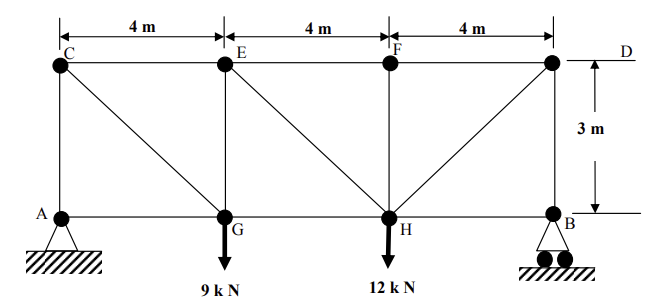
\includegraphics[width=0.8\columnwidth]{figs/ass3_d_q22.png}
    \caption{}
    \label{fig:placeholder}
\end{figure}

\begin{enumerate}
\item $AG$ is the only zero force member.
\item $AG$ and $BH$ are the only two zero force members.
\item $AG$, $BH$ and $HF$ are zero force members.
\item $AG$, $BH$, $HF$ and $GC$ are zero force members.
\end{enumerate}

(GATE XE 2016)

\end{enumerate}

\begin{center}
    \textbf{END OF SECTION - D}
\end{center}

\newpage

\begin{center}
    {\Large \textbf{E : THERMODYNAMICS}}
\end{center}

\textbf{Notation used: } 

$P$ – pressure, $V$ – volume, $T$ – temperature, $S$ – entropy, $H$ – enthalpy, $U$ – internal energy, $A$ – Helmholtz free energy, $C_p$ – specific heat capacity at constant pressure.  

Specific properties are designated by lower case symbols.  

\textbf{Useful data:}  

Universal gas constant $R = 8.314 \, \text{kJ/(kmol·K)}$  

$C_p$ of air $= 1.005 \, \text{kJ/(kg·K)}$  

Ratio of ideal gas specific heats for air: $\gamma = 1.4$  

Molecular mass of hydrogen: $2 \, \text{kg/kmol}$  



\begin{enumerate}

\item[] \textbf{Q. 1 – Q. 9 carry one mark each.}

\item Which of the following thermodynamic properties is NOT an intensive property of a thermodynamic system?

\begin{multicols}{2}
\begin{enumerate}
\item Pressure
\item Temperature
\item Density
\item Volume
\end{enumerate}
\end{multicols}

(GATE XE 2016)

\item An U-tube manometer shows a height difference of $z_1$ between the two columns for a known gauge pressure $P_1$ (both $z_1$ and $P_1$ in appropriate units). If the height difference between the two columns is $2z_1$, then the corresponding gauge pressure will be:

\begin{multicols}{4}
\begin{enumerate}
\item $P_1/2$
\item $2P_1$
\item $P_1$
\item $4P_1$
\end{enumerate}
\end{multicols}

(GATE XE 2016)

\item Water vapour can be treated as an ideal gas,

\begin{enumerate}
\item for all temperature and pressure
\item for sufficiently low pressure, regardless of its temperature
\item for very high pressure only
\item for sufficiently low temperature, regardless of its pressure
\end{enumerate}

(GATE XE 2016)

\item The thermal efficiency of a Carnot engine is $0.5$. If the temperature of the cold reservoir is $300 \, \text{K}$, then the temperature of the hot reservoir is:

\begin{multicols}{4}
\begin{enumerate}
\item 600 K
\item 1200 K
\item 900 K
\item 450 K
\end{enumerate}
\end{multicols}

(GATE XE 2016)

\item In a reversible, constant-pressure, non-flow process, heat input is given by

\begin{enumerate}
\item Change in internal energy
\item Change in enthalpy
\item Change in entropy
\item Work output
\end{enumerate}

(GATE XE 2016)

\item Moist air undergoes an adiabatic saturation process such that the relative humidity of air increases. For this process,

\begin{enumerate}
\item Dry bulb temperature increases, specific humidity increases
\item Dry bulb temperature increases, specific humidity decreases
\item Dry bulb temperature decreases, specific humidity increases
\item Dry bulb temperature decreases, specific humidity decreases
\end{enumerate}

(GATE XE 2016)

\item A steadily flowing ideal gas undergoes adiabatic throttling, where  
$T_1$: temperature before throttling  
$T_2$: temperature after throttling  
Assuming no change in kinetic and potential energy due to throttling, which of the following is correct:

\begin{multicols}{2}
\begin{enumerate}
\item $T_1 = T_2$
\item $T_1 > T_2$
\item $T_1 < T_2$
\item $T_1 = \gamma T_2, \ \gamma$: specific heat ratio
\end{enumerate}
\end{multicols}

(GATE XE 2016)

\item For irreversible heat transfer from a hot body to a cold body, if $\Delta$ denotes the property change of both hot and cold bodies (i.e. difference between its final and initial values), then

\begin{multicols}{2}
\begin{enumerate}
\item $\Delta S = 0$
\item $\Delta U > 0$
\item $\Delta S < 0$
\item $\Delta S > 0$
\end{enumerate}
\end{multicols}

(GATE XE 2016)

\item A closed system undergoes a cyclic process. For the net work done by the system on the surroundings, which of the following statements is FALSE:

\begin{enumerate}
\item Net work is always zero
\item Net work is $\oint P \, dV$ if the process is reversible
\item Net work can be negative
\item Net work can be positive
\end{enumerate}

(GATE XE 2016)

\item Consider the following statements related to the second law of thermodynamics:

P. A cyclic heat engine cannot produce net work by exchanging heat only with one reservoir.  

Q. The efficiency of a reversible heat engine is dependent on the nature and amount of working substance undergoing the cycle. 

R. It is impossible to have a cyclic device which will produce no effect other than the transfer of heat from a cold body to a hot body.  

S. It is impossible to have heat engines operating between a heat source and sink to have a lower efficiency than that of a reversible heat engine operating between the same source and sink.  

For which of the following options, BOTH the statements are inconsistent with the second law of thermodynamics:

\begin{multicols}{4}
\begin{enumerate}
\item P and R
\item P and Q
\item R and S
\item Q and S
\end{enumerate}
\end{multicols}

(GATE XE 2016)

\item[] \textbf{Q.10 - Q.22 carry two marks each.}

\item Consider the following statements related to air-standard Otto, Diesel, and Brayton cycles:

P. Brayton cycle has at least one isentropic and one isobaric process.  

Q. Otto cycle has at least one isentropic and one isochoric process.  

R. Diesel cycle has at least one isentropic and one isothermal process.  

S. At least one of the cycles has an isothermal process.  

For which of the following options, BOTH the statements are consistent with the operation of the above cycles:

\begin{multicols}{4}
\begin{enumerate}
\item P and R
\item P and Q
\item R and S
\item P and S
\end{enumerate}
\end{multicols}

(GATE XE 2016)

\item Volumetric analysis of a hydrocarbon combustion product shows 8\% CO$_2$, 15\% H$_2$O (vapour), 5.5\% O$_2$ and 71.5\% N$_2$. The combustion product flows steadily through a heat exchanger at 200 kPa pressure. Assume each component in the mixture to be an ideal gas. In order to avoid the condensation of H$_2$O in the heat exchanger, the minimum allowable temperature (in $^\circ$C) is \_\_\_\_\_\_. 


\begin{table}[H]
\centering
\caption{}
\label{}
\begin{tabular}{|c|c|c|c|c|c|}
\hline
$P$ (kPa) & 10 & 20 & 30 & 40 & 50 \\
\hline
$T$ ($^\circ$C) & 45.83 & 60.09 & 69.12 & 75.82 & 81.35 \\
\hline
\end{tabular}
\end{table}

(GATE XE 2016)

\item An equimolar mixture of two ideal gases (A, B) expands isentropically in a nozzle. The gas mixture enters the nozzle at 300 kPa, 400 K and exits at 100 kPa. Assuming the mixture to be an ideal gas, the exit temperature of the gas mixture (in K) is \_\_\_\_\_\_.


\begin{table}[H]
\centering
\caption{}
\label{}
\begin{tabular}{|c|c|c|}
\hline
 & Molar mass (kg/kmol) & $C_p$ (kJ/kg-K) \\
\hline
Gas A & 28.013 & 1.04 \\
\hline
Gas B & 2.016 & 14.21 \\
\hline
\end{tabular}
\end{table}

(GATE XE 2016)

\item A rigid vessel of volume 10 m$^3$ is filled with hydrogen at 25$^\circ$C and 500 kPa. Due to leakage, some gas has escaped from the vessel until the pressure in the vessel drops down to 200 kPa, and the corresponding temperature of the gas inside the vessel is found to be 15$^\circ$C. The amount of gas released (in kg) from the vessel is \_\_\_\_\_\_.

(GATE XE 2016)

\item A hot ideal gas ($C_p = 1.2$ kJ/kg-K) steadily flows through a turbine with inlet and exit temperatures of 1500 K and 500 K respectively. The minimum mass flow rate (in kg/s) of the hot gas to achieve a power output of 12 MW is \_\_\_\_\_\_.

(GATE XE 2016)

\item Air pressure inside a spherical balloon is proportional to its diameter. The balloon undergoes a reversible, isothermal, non-flow process. During the process, the balloon maintains its spherical shape, and the air inside the balloon consumes 2 kJ of heat. Initial air pressure inside the balloon was 120 kPa, while the initial balloon diameter was 20 cm. Assuming air to be an ideal gas, the final diameter of the balloon (in cm) is \_\_\_\_\_\_.

(GATE XE 2016)

\item An air-standard diesel engine has a compression ratio of 18 (the ratio of the volume at the beginning of the compression process to that at the end of the compression process), and a cut-off ratio of 2 (the ratio of the volume at the end of the heat addition process to that at the beginning of the heat addition process). The thermal efficiency (in \%) of the engine is \_\_\_\_\_\_.

(GATE XE 2016)

\item Compressed air, at 1 MPa pressure, 400 K temperature flows through a large pipe. An evacuated, insulated rigid tank of 0.5 m$^3$ volume is connected to the pipe through a valve. The valve is opened to fill the tank and the valve closes automatically when the tank pressure reaches 1 MPa. Assuming ideal gas behavior, the final air temperature in the tank (in K) is \_\_\_\_\_\_.

(GATE XE 2016)

\item A 40 kg metal block ($C_p = 0.5$ kJ/kg-K) at $T_i = 450^\circ$C is quenched in 150 kg oil ($C_p = 2.5$ kJ/kg-K) at $T = 25^\circ$C. If the combined (metal block and oil) system is fully isolated from its surroundings, then the net change in the entropy (in kJ/K) of the combined system is \_\_\_\_\_\_.

(GATE XE 2016)

\item For phase change from solid (sol) to liquid (liq) state, if the slope of the solid-liquid coexistence line in the $P$-$T$ diagram is negative, then:
\begin{multicols}{4}
\begin{enumerate}
\item $v_{liq} < v_{sol}$
\item $v_{liq} > v_{sol}$
\item $s_{liq} < s_{sol}$
\item $h_{liq} < h_{sol}$
\end{enumerate}
\end{multicols}
(GATE XE 2016)

\item A house-hold refrigerator operates under steady state condition between an evaporator temperature of $263 \, K$ and a condenser temperature of $323 \, K$. The heat load to the refrigerator is $3 \, kW$. The actual COP of the refrigerator is half of that of a Carnot refrigerator operating between the same condenser and evaporator temperatures. The power required (in kW) to run the refrigerator is \_\_\_\_\_\_\_

(GATE XE 2016)

\item The Maxwell relation that results from the expression for the Helmholtz free energy $A = U - TS$, is:
\begin{multicols}{2}
\begin{enumerate}
\item $\left(\frac{\partial T}{\partial v}\right)_{S} = - \left(\frac{\partial P}{\partial S}\right)_{v}$
\item $\left(\frac{\partial T}{\partial P}\right)_{S} = \left(\frac{\partial v}{\partial S}\right)_{P}$
\item $\left(\frac{\partial P}{\partial T}\right)_{v} = \left(\frac{\partial S}{\partial v}\right)_{T}$
\item $\left(\frac{\partial v}{\partial T}\right)_{P} = - \left(\frac{\partial S}{\partial P}\right)_{T}$
\end{enumerate}
\end{multicols}

(GATE XE 2016)


\end{enumerate}

\begin{center}
    \textbf{END OF SECTION - E}
\end{center}

\newpage

\begin{center}
    {\Large \textbf{F : POLYMER SCIENCE AND ENGINEERING}}
\end{center}

\begin{enumerate}

\item[] \textbf{Q.1 - Q.9 carry one mark each.}

\item The polymer with minimum number of branches is
\begin{multicols}{2}
\begin{enumerate}
\item HDPE 
\item VLDPE 
\item LDPE 
\item LLDPE 
\end{enumerate}
\end{multicols}
(GATE XE 2016)

\item Nitrile rubber is a copolymer of
\begin{multicols}{2}
\begin{enumerate}
\item isoprene and acrylonitrile 
\item butadiene and acrylonitrile 
\item cyclopentadiene and acrylonitrile 
\item isobutylene and acrylonitrile 
\end{enumerate}
\end{multicols}
(GATE XE 2016)

\item The functionality of 1,4-divinylbenzene in reactions involving addition across carbon-carbon double bond is
\begin{multicols}{4}
\begin{enumerate}
\item 1 
\item 2 
\item 3 
\item 4 
\end{enumerate}
\end{multicols}
(GATE XE 2016)

\item The comonomer common to Nylon 66 and Nylon 46 is
\begin{multicols}{2}
\begin{enumerate}
\item hexamethylene diamine 
\item butylene diamine 
\item adipic acid 
\item octane dicarboxylic acid 
\end{enumerate}
\end{multicols}
(GATE XE 2016)

\item Polyethylene and polypropylene form an immiscible blend mainly due to
\begin{multicols}{2}
\begin{enumerate}
\item entropy factor 
\item enthalpy factor 
\item crystallinity 
\item solubility 
\end{enumerate}
\end{multicols}
(GATE XE 2016)

\item Rubber modulus is
\begin{multicols}{2}
\begin{enumerate}
\item ratio of stress to strain 
\item same as Young's modulus 
\item stress at specified strain 
\item stress at break 
\end{enumerate}
\end{multicols}
(GATE XE 2016)

\item The solubility parameter is determined by using
\begin{multicols}{2}
\begin{enumerate}
\item Bragg's equation 
\item Fox equation 
\item Hildebrand equation 
\item Carother's equation 
\end{enumerate}
\end{multicols}
(GATE XE 2016)

\item ‘Roller die’ consists of a combination of
\begin{enumerate}
\item a two-roll calender with internal mixer feeding 
\item a two-roll calender with open mill feeding 
\item a three-roll vertical calender with two-roll mixer feeding 
\item a two-roll calender with extruder feeding 
\end{enumerate}
(GATE XE 2016)

\item Resole is an example of
\begin{multicols}{2}
\begin{enumerate}
\item thermoplastic polymer 
\item thermosetting polymer 
\item natural polymer 
\item thermoplastic elastomer 
\end{enumerate}
\end{multicols}
(GATE XE 2016)

\item[] \textbf{Q.10 - Q.22 carry two marks each.}

\item Match the processing technique to the appropriate product listed below:  

\begin{table}[H]
\centering
\begin{tabular}{|c|c|}
\hline
\textbf{Processing Technique} & \textbf{Product} \\ \hline
P. Blow molding & 1. Bucket \\ \hline
Q. Co-extrusion & 2. Blister packaging \\ \hline
R. Injection molding & 3. Bottles \\ \hline
S. Thermoforming & 4. Multilayered sheets \\ \hline
\end{tabular}
\caption{}
\label{}
\end{table}

\begin{multicols}{2}
\begin{enumerate}
\item P:3, Q:4, R:2, S:1
\item P:3, Q:1, R:4, S:2
\item P:3, Q:4, R:1, S:2
\item P:3, Q:2, R:1, S:4
\end{enumerate}
\end{multicols}
(GATE XE 2016)

\item For a high molecular weight polymer sample with a viscosity of $6 \times 10^{11}$ Poise and a stress relaxation modulus of $3 \times 10^{6}$ dyne cm$^{-2}$ at a given temperature, the relaxation time will be \_\_\_\_ hours.  

(GATE XE 2016)

\item Match the following polymer additives to their function:  

\begin{table}[H]
\centering
\begin{tabular}{|c|c|}
\hline
\textbf{Additive} & \textbf{Function} \\ \hline
P. Azocarbonamide & 1. Chemical plasticizer \\ \hline
Q. Antimony trioxide & 2. Accelerator \\ \hline
R. Pentachlorothiophenol & 3. Flame retardant \\ \hline
S. Mercaptobenzothiazole & 4. Blowing agent \\ \hline
\end{tabular}
\caption{}
\label{}
\end{table}

\begin{multicols}{2}
\begin{enumerate}
\item P:4, Q:1, R:3, S:2
\item P:4, Q:2, R:1, S:3
\item P:4, Q:3, R:2, S:1
\item P:4, Q:3, R:1, S:2
\end{enumerate}
\end{multicols}
(GATE XE 2016)

\item Tensile force of $165$ N is applied to a piece of vulcanized rubber of dimension $4$ mm $\times$ $4$ mm $\times$ $30$ mm. If the sample is elongated by 50\% of its original length under the same applied force, the true stress will be \_\_\_\_ MPa.  

(GATE XE 2016)

\item The order of glass transition temperature for the given polymers is 

[NR = natural rubber; PP = polypropylene; PE = polyethylene; PMMA = poly(methyl methacrylate)]  

\begin{enumerate}
\item NR $<$ PE $<$ PP $<$ PMMA
\item PE $<$ NR $<$ PP $<$ PMMA
\item PP $<$ NR $<$ PE $<$ PMMA
\item NR $<$ PP $<$ PE $<$ PMMA
\end{enumerate}
(GATE XE 2016)

\item Dynamic mechanical analysis of polystyrene ($T_g=100\,^\circ$C) measured at a frequency of 1 Hz shows the damping peak at 110$^\circ$C. If the measurement is made at 10 Hz, then the peak temperature ($^\circ$C) will be  

\begin{multicols}{4}
\begin{enumerate}
\item 123.2
\item 133.2
\item 143.2
\item 153.2
\end{enumerate}
\end{multicols}
(GATE XE 2016)

\item Match the product to the most suitable plastic listed below:  

\begin{table}[H]
\centering
\begin{tabular}{|c|c|}
\hline
\textbf{Product} & \textbf{Plastic} \\ \hline
P. Baby feeding bottle & 1. Polypropylene \\ \hline
Q. Tiffin box & 2. Poly(ethylene terephthalate) \\ \hline
R. Water bottle & 3. Poly(vinyl chloride) \\ \hline
S. Blood bag & 4. Polycarbonate \\ \hline
\end{tabular}
\caption{}
\label{}
\end{table}

\begin{multicols}{2}
\begin{enumerate}
\item P:1, Q:4, R:2, S:3
\item P:4, Q:1, R:2, S:3
\item P:1, Q:3, R:2, S:4
\item P:4, Q:3, R:2, S:1
\end{enumerate}
\end{multicols}
(GATE XE 2016)

\item The number average molecular weight for the polymerization of adipic acid and ethylene glycol (feed ratio 1:1) at 99 percent conversion is \_\_\_\_\_ g mol$^{-1}$. 

(GATE XE 2016)

\item A composite material contains 30 \% by volume of uniaxially aligned glass fibres in a matrix of alkyd resin. The tensile moduli of the glass fibre and alkyd resin are 76 GPa and 3 GPa, respectively. If a tensile stress of 100 MPa is applied parallel to the fibres, the percentage longitudinal strain is \_\_\_\_\_. 

(GATE XE 2016)

\item Match the elastomers listed below to the appropriate curing agent:

\begin{table}[H]
\centering
\begin{tabular}{|c|c|}
\hline
Elastomer & Curing Agent \\
\hline
P. Silicone rubber & 1. Zinc oxide + ethylene thiourea \\
Q. Natural rubber & 2. Diamine \\
R. Chloroprene rubber & 3. Sulfur \\
S. Acrylate elastomer & 4. Dicumyl peroxide \\
\hline
\end{tabular}
\end{table}

\begin{multicols}{2}
\begin{enumerate}
\item P:4, Q:3, R:1, S:2
\item P:3, Q:4, R:1, S:2
\item P:4, Q:1, R:3, S:2
\item P:2, Q:3, R:4, S:1
\end{enumerate}
\end{multicols}
(GATE XE 2016)

\item The weight of graphite fiber (density $=1800 \,\text{kg m}^{-3}$) that should be added to 1.00 kg of vinyl ester resin (density $=1250 \,\text{kg m}^{-3}$) to produce a composite with a density of $1600 \,\text{kg m}^{-3}$ is \_\_\_\_\_ kg. 

(GATE XE 2016)

\item If the values of $K$ and $a$ in the Mark–Houwink equation are $1.5 \times 10^{-4}$ dL g$^{-1}$ and 0.60, respectively, the viscosity average molecular weight of a polymer having an intrinsic viscosity of 0.05 dL g$^{-1}$ is \_\_\_\_\_ kg mol$^{-1}$. 

(GATE XE 2016)

\item A rectangular polymer bar of length 40 mm fits exactly into a steel mold cavity and the entire assembly was heated from 20 to 100 $^\circ$C. The linear thermal expansion coefficients of the polymer and steel are $80 \times 10^{-6}$ $^\circ$C$^{-1}$ and $11 \times 10^{-6}$ $^\circ$C$^{-1}$, respectively. The strain encountered by the polymer sample along the length will be \_\_\_\_\_ \%. 

(GATE XE 2016)

\end{enumerate}

\begin{center}
    \textbf{END OF SECTION - F}
\end{center}

\newpage

\begin{center}
    {\Large \textbf{G : FOOD TECHNOLOGY}}
\end{center}

\begin{enumerate}

\item[] \textbf{Q.1 - Q.9 carry one mark each.}

\item Bread staling is caused by \_\_\_\_\_
\begin{multicols}{4}
\begin{enumerate}
\item Caramelisation
\item Gelatinisation
\item Retrogradation
\item Aggregation
\end{enumerate}
\end{multicols}
(GATE XE 2016)

\item Arrange the grades of tea in the increasing order of their leaf size \_\_\_\_, \_\_\_\_ and \_\_\_\_.
\begin{enumerate}
\item Souchang, pekoe and orange pekoe
\item Pekoe, souchang and orange pekoe
\item Orange pekoe, souchang, and pekoe
\item Orange pekoe, pekoe, and souchang
\end{enumerate}
(GATE XE 2016)

\item Fruit juice is being pasteurized in a tubular heat exchanger. The retention time in holding tube of $0.2 \, m^2$ cross sectional area is $3$ seconds. If the flow rate of juice is $0.4 \, m^3 s^{-1}$, the length of the holding tube in m, is \_\_\_\_\_\_\_.

(GATE XE 2016)

\item The oil, which experiences flavor reversion even at the lower peroxide value is \_\_\_\_
\begin{multicols}{2}
\begin{enumerate}
\item Mustard
\item Soybean
\item Palm
\item Sesame
\end{enumerate}
\end{multicols}
(GATE XE 2016)

\item 80 kg of wheat containing 10 kg of moisture has been dried to a moisture content of $8\%$ wet basis in 3 hours under constant rate period of drying. The drying rate in $kg \, h^{-1}$ is \_\_\_\_

(GATE XE 2016)

\item The rate of cream separation in a disc bowl centrifuge can be increased by \_\_\_\_
\begin{multicols}{2}
\begin{enumerate}
\item Increasing the size of the bowl
\item Lower viscosity of fluid
\item Increasing RPM of the bowl
\item All of these
\end{enumerate}
\end{multicols}
(GATE XE 2016)

\item Which one of the following is not used in mass transfer analysis?
\begin{multicols}{2}
\begin{enumerate}
\item Biot number
\item Peclet number
\item Schmidt number
\item Sherwood number
\end{enumerate}
\end{multicols}
(GATE XE 2016)

\item Oxygen is permeating through an EVOH film of thickness $t$ and solubility coefficient $S$. If diffusivity of oxygen through the film is $D$, then permeability of oxygen through the film will be \_\_\_\_
\begin{multicols}{4}
\begin{enumerate}
\item $D/t$
\item $D/S$
\item $D \times S$
\item $S/D$
\end{enumerate}
\end{multicols}
(GATE XE 2016)

\item Condensing steam is used to heat vegetable oil in a double pipe co-current heat exchanger. If the inlet and outlet temperature of steam are $T_{hi}$ and $T_{ho}$, and for vegetable oil $T_{ci}$ and $T_{co}$, respectively, the log mean temperature difference $(\Delta T_{LM})$ will be
\begin{multicols}{2}
\begin{enumerate}
\item $\dfrac{T_{hi}-T_{co}}{\ln \dfrac{T_{hi}-T_{co}}{T_{ho}-T_{ci}}}$
\item $\dfrac{(T_{ho}-T_{ci})-(T_{hi}-T_{co})}{\ln \dfrac{T_{ho}-T_{ci}}{T_{hi}-T_{co}}}$
\item $\dfrac{(T_{hi}-T_{co})-(T_{ho}-T_{ci})}{\ln \dfrac{T_{hi}-T_{co}}{T_{ho}-T_{ci}}}$
\item $\dfrac{T_{co}-T_{ci}}{\ln \dfrac{T_{hi}-T_{ci}}{T_{ho}-T_{co}}}$
\end{enumerate}
\end{multicols}
(GATE XE 2016)

\item[] \textbf{Q. 10 – Q. 22 carry two marks each. }

\item Match the food spoilage organisms given in Column I with the associated foods given in Column II

\begin{table}[H]
\centering
\begin{tabular}{ll}
\textbf{Column I} & \textbf{Column II} \\
P. Clostridium botulinum & 1. Fish \\
Q. Salmonella spp. & 2. Cooked starch foods \\
R. Vibrio parahaemolyticus & 3. Meat, egg and poultry \\
S. Bacillus cereus & 4. Canned foods \\
\end{tabular}
\caption{}
\label{}
\end{table}

\begin{multicols}{2}
\begin{enumerate}
\item P-4, Q-3, R-1, S-2
\item P-3, Q-4, R-2, S-1
\item P-2, Q-1, R-3, S-4
\item P-4, Q-3, R-2, S-1
\end{enumerate}
\end{multicols}
(GATE XE 2016)

\item Fluid is flowing inside a pipe of radius $R$ in fully developed laminar flow. If the velocity of the fluid at the centre at a distance $L$ is $v_{\max}$, velocity at radial distance of $\tfrac{3}{4}(R)$ will be $\_\_\_\_$ times $v_{\max}$

\begin{multicols}{4}
\begin{enumerate}
\item 9/16
\item 7/16
\item 16/9
\item 16/7
\end{enumerate}
\end{multicols}
(GATE XE 2016)

\item A meat ball with a radius of 25.4 mm at a temperature of 700 K, is suddenly plunged into a medium whose temperature is held at 395 K. Assume a convective heat transfer coefficient of $11.5 \; W \, m^{-2} \, K^{-1}$ and take the average physical properties as: $K = 44 \, W \, m^{-1} \, K^{-1}$, $\rho = 7850 \, kg \, m^{-3}$ and $c_p = 0.4606 \, kJ \, kg^{-1} \, K^{-1}$. The temperature (K) of the meat ball after one hour is $\_\_\_\_$

(GATE XE 2016)

\item a) Assertion: Acidulates are added in soft drinks to provide a buffering action.

r) Reason: Buffers tend to prevent changes in pH and prevent excessive tartness.

Choose the correct answer from the following

\begin{enumerate}
\item Both a) and r) are true but r) is not the correct reason
\item Both a) and r) are true and r) is the correct reason for a)
\item a) is true but r) is false
\item Both a) and r) are false
\end{enumerate}
(GATE XE 2016)

\item The $D_{121}$ and $z$ values for \textit{C. botulinum} spores in canned food are 0.2 min and 10 $^{\circ}$C respectively. Total time required in min, to reduce the spores from $10^{2}$ to $10^{-6}$ at 111 $^{\circ}$C is $\_\_\_\_$

(GATE XE 2016)

\item a) Assertion: Olestra is used as a zero calorie fat replacer 

r) Reason: It is a sucrose polyester with 6--8 acyl group and is not absorbed in the human digestive system. 

Choose the correct answer from the following

\begin{enumerate}
\item Both a) and r) are true and r) is the correct reason for a)
\item Both a) and r) are true, but r) is not the correct reason for a)
\item a) is true but r) is false
\item Both a) and r) are false
\end{enumerate}

(GATE XE 2016)

\item Match the enzymes in Column I with their functions in Column II \\
\begin{table}[h]
\centering
\begin{tabular}{ll}
\textbf{Column I} & \textbf{Column II} \\
P. Amylase & 1. Conversion of sucrose to glucose and fructose \\
Q. Invertase & 2. Softening of dough \\
R. Phosphatase & 3. Effectiveness of pasteurization \\
S. Protease & 4. Conversion of starch to maltose \\
\end{tabular}
\caption{}
\label{}
\end{table}
\begin{multicols}{2}
\begin{enumerate}
\item P-1, Q-2, R-3, S-4
\item P-4, Q-1, R-3, S-2
\item P-1, Q-4, R-2, S-3
\item P-2, Q-4, R-3, S-1
\end{enumerate}
\end{multicols}
(GATE XE 2016)

\item Match the terms in Column I with their most appropriate description in Column II \\
\begin{table}[h]
\centering
\begin{tabular}{ll}
\textbf{Column I} & \textbf{Column II} \\
P. Enrichment & 1. Overcome the deficiency of nutrient by mixing of two plant sources \\
Q. Fortification & 2. Overcome the deficiency of nutrient from a synthetic source \\
R. Supplementation & 3. Restoration of nutrient which is lost during processing \\
S. Complementation & 4. Addition of nutrient which may or may not originally present \\
\end{tabular}
\caption{}
\label{}
\end{table}
\begin{multicols}{2}
\begin{enumerate}
\item P-3, Q-4, R-2, S-1
\item P-1, Q-2, R-3, S-4
\item P-1, Q-4, R-3, S-2
\item P-2, Q-3, R-1, S-4
\end{enumerate}
\end{multicols}
(GATE XE 2016)

\item Match the products in Column I with their Original Phase in Column II \\
\begin{table}[h]
\centering
\begin{tabular}{ll}
\textbf{Column I} & \textbf{Column II} \\
P. Milk & 1. Colloidal \\
Q. Butter & 2. Solution \\
R. Lactose & 3. Water in oil emulsion \\
S. Casein & 4. Oil in water emulsion \\
\end{tabular}
\caption{}
\label{}
\end{table}
\begin{multicols}{2}
\begin{enumerate}
\item P-3, Q-4, R-1, S-2
\item P-3, Q-4, R-2, S-1
\item P-4, Q-3, R-2, S-1
\item P-4, Q-3, R-1, S-2
\end{enumerate}
\end{multicols}
(GATE XE 2016)

\item a) Assertion: Presence of low sulphur containing amino acids make casein in milk to boil, sterilize and concentrate without coagulation even at higher temperature. 

r) Reason: This is due to the restricted formation of di-sulphide bonds resulting in increased stability. 

Choose the correct answer from the following

\begin{enumerate}
\item Both a) and r) are true and r) is the correct reason for a)
\item Both a) and r) are true but r) is not the correct reason for a)
\item Both a) and r) are false
\item a) is true but r) is false
\end{enumerate}

(GATE XE 2016)

\item In a typical Psychrometric Chart shown below, the processes OP, OQ and OR related to air water vapor mixture are \_\_\_\_, \_\_\_\_ and \_\_\_\_.

\begin{figure}[H]
    \centering
    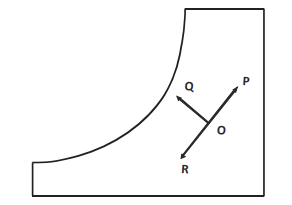
\includegraphics[width=0.5\columnwidth]{figs/ass3_g_q20.png}
    \caption{}
    \label{fig:placeholder}
\end{figure}

\begin{enumerate}
\item Cooling \& dehumidification, cooling \& humidification, heating \& humidification
\item Cooling \& dehumidification, heating \& humidification, drying
\item Heating \& humidification, cooling \& humidification, cooling \& dehumidification
\item Heating \& humidification, cooling \& dehumidification, drying
\end{enumerate}

(GATE XE 2016)

\item A fruit juice with a negligible boiling point rise is being evaporated using saturated steam at $121.1\,^{\circ}\mathrm{C}$ in a triple effect evaporator having equal area in each effect. The pressure of the vapor in the last effect is $25.6$ kPa absolute and the corresponding saturation temperature is $65.7\,^{\circ}\mathrm{C}$. The heat transfer coefficients are $U_1 = 2760, U_2 = 1875$ and $U_3 = 1350$ W m$^{-2}$ K$^{-1}$. The boiling point ($^{\circ}$C) in the first effect is \_\_\_\_.

(GATE XE 2016)

\item In an aeration system, $520$ kg of wheat grains having average size of $0.15$ mm, shape factor of $0.88$ and density of $1040$ kg m$^{-3}$ are fluidized using air at $2$ atm absolute and $25\,^{\circ}\mathrm{C}$. If the cross section of empty bed is $0.4$ m$^{2}$, the minimum height (m) of the fluidized bed, with voidage of $0.45$ will be \_\_\_\_. 

(GATE XE 2016)


\end{enumerate}

\begin{center}
    \textbf{END OF QUESTION PAPER}
\end{center}

\end{document}

